\documentclass[useAMS,usenatbib]{mn2e}
\usepackage{graphicx}
\usepackage{hyperref}
\usepackage{tikz}
\usetikzlibrary{calc,fadings,decorations.pathreplacing}
%\usepackage{url}
\newcommand{\aj}{Astron. J.}
\newcommand{\apj}{Astrophys. J.}
\newcommand{\pasp}{Publ. Ast. Soc. Pac.}
\newcommand{\pasa}{Publ. Ast. Soc. Aust.}
\newcommand{\ao}{Appl. Opt.}


\newcommand\pgfmathsinandcos[3]{%
  \pgfmathsetmacro#1{sin(#3)}%
  \pgfmathsetmacro#2{cos(#3)}%
}
\newcommand\LongitudePlane[3][current plane]{%
  \pgfmathsinandcos\sinEl\cosEl{#2} % elevation
  \pgfmathsinandcos\sint\cost{#3} % azimuth
  \tikzset{#1/.style={cm={\cost,\sint*\sinEl,0,\cosEl,(0,0)}}}
}
\newcommand\LatitudePlane[3][current plane]{%
  \pgfmathsinandcos\sinEl\cosEl{#2} % elevation
  \pgfmathsinandcos\sint\cost{#3} % latitude
  \pgfmathsetmacro\yshift{\cosEl*\sint}
  \tikzset{#1/.style={cm={\cost,0,0,\cost*\sinEl,(0,\yshift)}}} %
}
\newcommand\DrawLongitudeCircle[2][1]{
  \LongitudePlane{\angEl}{#2}
  \tikzset{current plane/.prefix style={scale=#1}}
   % angle of "visibility"
  \pgfmathsetmacro\angVis{atan(sin(#2)*cos(\angEl)/sin(\angEl))} %
  \draw[current plane] (\angVis:1) arc (\angVis:\angVis+180:1);
  \draw[current plane,dashed] (\angVis-180:1) arc (\angVis-180:\angVis:1);
}

\newcommand\DrawHalfLongitudeCircle[2][1]{
  \LongitudePlane{\angEl}{#2}
  \tikzset{current plane/.prefix style={scale=#1}}
   % angle of "visibility"
  \pgfmathsetmacro\angVis{atan(sin(#2)*cos(\angEl)/sin(\angEl))} %
  \draw[current plane] (\angVis:1) arc (\angVis:\angVis+90:1);
%  \draw[current plane,dashed] (\angVis:1) arc (\angVis-90:\angVis:1);
}
\newcommand\DrawLatitudeCircle[2][1]{
  \LatitudePlane{\angEl}{#2}
  \tikzset{current plane/.prefix style={scale=#1}}
  \pgfmathsetmacro\sinVis{sin(#2)/cos(#2)*sin(\angEl)/cos(\angEl)}
  % angle of "visibility"
  \pgfmathsetmacro\angVis{asin(min(1,max(\sinVis,-1)))}
  \draw[current plane] (\angVis:1) arc (\angVis:-\angVis-180:1);
  \draw[current plane,dashed] (180-\angVis:1) arc (180-\angVis:\angVis:1);
}

%% document-wide tikz options and styles

\tikzset{%
  >=latex, % option for nice arrows
  inner sep=0pt,%
  outer sep=2pt,%
  mark coordinate/.style={inner sep=0pt,outer sep=0pt,minimum size=3pt,
    fill=black,circle}%
}

\title[FermiFAST]{FermiFAST: A Fast Algorithm for Finding Point Sources
in the Fermi Data Stream}
\author[J. S. Heyl, A. Ashathaman and A. Barton]{Jeremy S. Heyl$^{1}$\thanks{Email:
    heyl@phas.ubc.ca; Canada Research Chair}, Asha Ashathaman and Alistair Barton\\
$^{1}$Department of Physics and Astronomy, University of British
Columbia, 6224 Agricultural Road, Vancouver, BC V6T 1Z1, Canada}


\begin{document}
\date{Accepted ---. Received ---; in original form ---}

\pagerange{\pageref{firstpage}--\pageref{lastpage}} \pubyear{2015}

\maketitle

\label{firstpage}

\begin{abstract}
  This paper presents new and efficient algorithms for finding point
  sources in the photon event data stream from the 
  Fermi Gamma-Ray Space Telescope.
\end{abstract}

\begin{keywords}
methods: data analysis --- methods: observational --- techniques:
image processing --- astrometry
\end{keywords}

\section{Introduction}

\section{The Photon Database}

The key to the speed of this algorithm is the database that contains
the position of the observed photons on the sky.  Each photon is
stored in a four-dimensional $k-d$~tree
\citep{Bentley:1975:MBS:361002.361007}.  We use the particularly
memory efficient implementation of \citet{LangPhD} (used in
astrometry.net).  The coordinates are actually stored as shorts
instead of floats to save additional memory.  The typical coordinates
range from $-1$ to $+1$, so using shorts yields an angular precision
of about six arcseconds much finer than that of the Fermi point-spread
function (PSF).  This memory efficient implementation allows us to
store all of the photons detected by Fermi above 100~MeV and within a
zenith angle of 100 degrees in memory simulataneously.

The first three dimensions contain the position of the photon on the
celestial sphere as shown in the upper portion of
Fig.~\ref{fig:sphere}.  Storing the direction of the photon momentum
in this manner removes the coordinate singularity of the spherical
coordinates.  Additionally it makes integrating over the celestial
sphere straightforward because $\int d\Omega = \int 2\pi \delta p d
\delta p$ where $\delta {\bf p} = {\bf p}' - {\bf p}$ is the three
dimensional vector between two points on the sphere.  The fourth
coordinate that we denote by $w$ depends on the point-spread function
for the photon in question.  In particular $w=\pm
\sqrt{R^2_\mathrm{max}-R_i^2}$ where $R_i$ is the radius of the
ninety-fifth percentile at the energy, entrance angle and front or
back conversion for the photon.  For convenience we use positive
values of $w$ for front-converted photons and negative values of $w$
for back-converted photons.  Furthermore, $R_\mathrm{max}$ is the
ninety-fifth percentile for the photon with the poorest angular
resolution.  This is depicted in the lower panel of
Fig.~\ref{fig:sphere}.
\begin{figure}
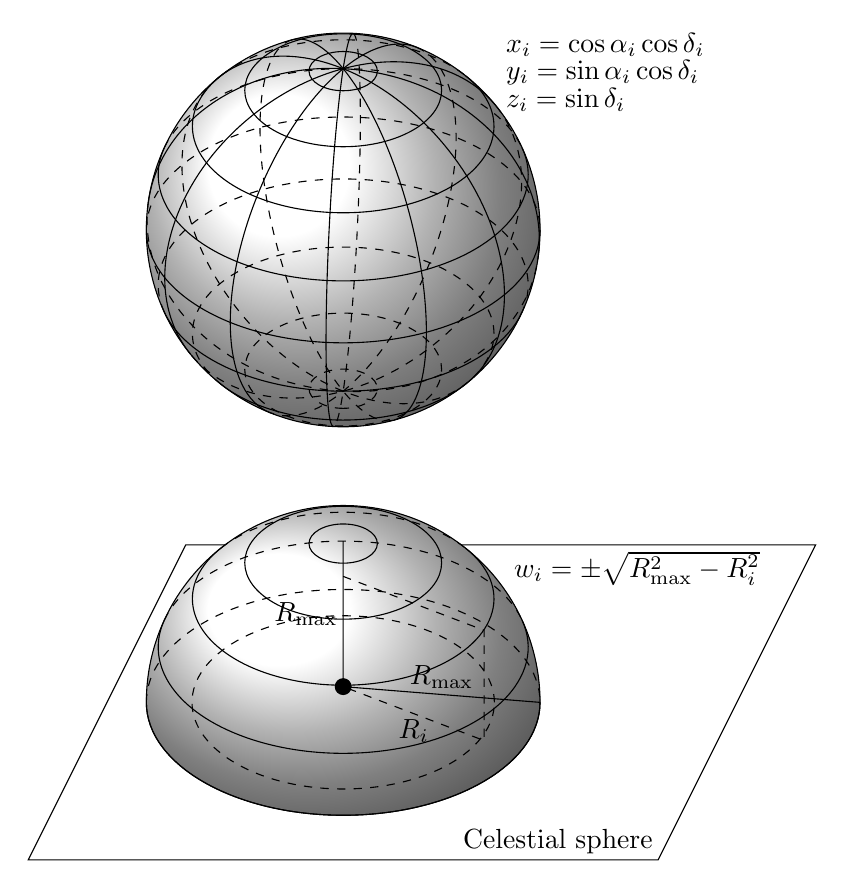
\begin{tikzpicture} % "THE GLOBE" showcase

\def\R{2.5} % sphere radius
\def\angEl{35} % elevation angle
\filldraw[ball color=white] (0,0) circle (\R);
\foreach \t in {-80,-60,...,80} { \DrawLatitudeCircle[\R]{\t} }
\foreach \t in {-5,-35,...,-175} { \DrawLongitudeCircle[\R]{\t} }
\draw (2,2.35) node [right] {$x_i=\cos\alpha_i\cos\delta_i$} 
      (2,2.0) node [right] {$y_i=\sin\alpha_i\cos\delta_i$}
      (2,1.65) node [right] {$z_i=\sin\delta_i$};
\begin{scope}[shift={(0,-6)}]
\draw (-4,-2) -- (-2,2) -- (6,2) -- (4,-2) -- cycle;
\draw (4,-2) node [above left] {Celestial sphere};
\filldraw[ball color=white] (0:\R) arc (0:180:\R)
(0,0) (0:\R) arc (0:-180:2.5 and 1.433904196);
\foreach \t in {0,20,...,80} { \DrawLatitudeCircle[\R]{\t} }
\draw (2.1,1.7) node [right] {$w_i=\pm\sqrt{R^2_\mathrm{max}-R^2_i}$};
\draw (0,0.2) -- node [above] {$R_\mathrm{max}$} (\R,0)
      (0,0.2) -- node [left] {$R_\mathrm{max}$} (0,0.81916*\R);
\draw [dashed] (0,1.6) -- ++(1.79,-0.6855) -- ++(0,-1.4) 
      -- node [below] {$R_i$} (0,0.2)
      (0,0.0) circle (1.92 and 1.10);
\filldraw[black] (0,0.2) circle (0.1);
\end{scope}
\end{tikzpicture}
\caption{The location of a given photon event on the celestial sphere
  and in the additional dimension. $R_i$ is the ninety-fifth
  percentile radius for the photon in question and $R_\mathrm{max}$ is
  the largest ninety-fifth percentile radius for the photons in the
  sample.}
\label{fig:sphere}
\end{figure}

Once the $k-d$~tree is created, it is efficient to find all of the
entries within the database within a given Cartesian distance of a
particular point.  In our case we query the database for all of the
photons within a distance $R_\mathrm{max}$ of a particular point on
the celestial sphere and use $w=0$ for the fourth coordinate.  The
particular choice of $w$ for the observed photons means that the query
will yield all of the photons that are within the ninety-fifth
percentile of the PSF.  In other words, if there is a point source
located at that particular point the query will return on average 95\%
of the photons from that source.  Of course, it will also return
photons from the background and other nearby sources.  This means that
the region of interest for a particular prospective source is energy
dependent.  The form of the exposure map also is energy dependent as
shown in Fig.~\ref{fig:expmap}.  It peaks at 0.95 times the exposure
time in the direction of the potential source and slowly drops to the
ninety-fifth percentile of the PSF in radius and then drops according
to the power-law of the tail component of the linear combinations of
King function that are used to characterize the Fermi PSF. 
\begin{figure}
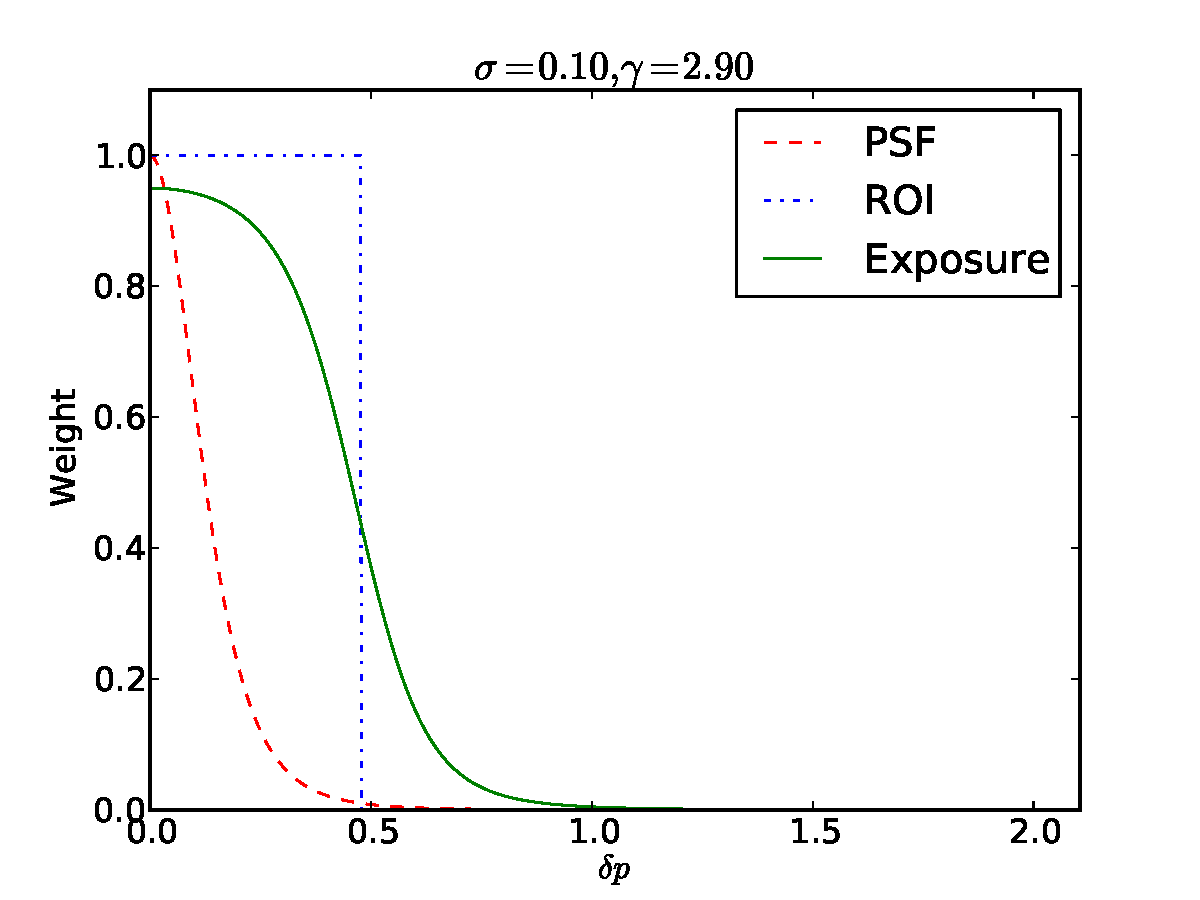
\includegraphics[width=\columnwidth]{expmap}
\caption{The Exposure Map, Region of Interest (ROI)
  and Point-Spread Function (PSF)}
\label{fig:expmap}
\end{figure}

Altough the construction of the tree is not done in parallel, the
queries are performed in parallel using the tree held in shared
memory.  For example if one uses all the photons above 100~MeV from
weeks 9 through 316 with a standard zenith angle cut (89,684,009
photons) requires one gigabyte to store the tree and about ten minutes
to construct.  The 200,000 location queries and likelihood
calculations require 140,000 seconds (700~ms each), so the
speed-up through parallisation can be dramatic.  On the other hand, if
one restricts to photons above 1~GeV (13,193,171), it only takes 90
seconds to construct the tree.  At higher energies, it makes sense to
make more location queries because the PSF is smaller.  In this
example 786,426 queries require 5,600 seconds of CPU time (7~ms each)
or only six minutes on sixteen cores.

\section{Source Likelihood}

Using the $k-d$~tree to determine the photons that would like within
the 95\% enclosure region of the point-spread function, we calculate
several statistics of the observed photons to assess the likelihood of
a source being at a particular position on the sky.  We first
determine two statistics whose distributions are known. First, if all
of the photons within the region of interest (all photons that lie
within the 95th-percentile cone of the potential source) indeed come
from a uniform background, the ratio of the solid angle enclosed in a
circle centred on the potential source and running through the
observed to the total solid angle within the region of interest for
that particular photon should be uniformly distributed between zero
and one.  We denote the mean of this ratio over the observed photons
$\bar r^2$.  This is a Bates distribution with mean of $1/2$ and
variance of $1/(12 N_\mathrm{photons})$.  Second, if all of the photons within the
region of interest indeed come from a point source at the centre of
the region of interest, the ratio of the percentile of a given photon
within the cumulative PSF distribution for that particular photon to
0.95 should be uniformly distributed between zero and one.  We denote
this statistic by $\bar f$.

If we assume that the observed photons originate from a linear
combination of these two possiblities, we can determine the ratio of
the two contributions from these statistics. In particular the fraction
of photons that come from the point source would be
\begin{equation}
  A_f=\frac{\frac{1}{2}-\bar r^2}{\bar f-\bar r^2}
  \label{eq:1}
\end{equation}
and we can estimate the significance of the value of $A_f$ by
\begin{equation}
  S(r^2) = \left ( \bar r^2-\frac{1}{2} \right ) \sqrt{12 N_\mathrm{photons}}
\end{equation}
and the probabilty of getting a value of $S(r^2)$ larger than $x$ by
chance is
\begin{equation}
  P\left [ S(r^2) > x \right ] = \frac{1}{2} \mathrm{erfc} \left ( \frac{x}{\sqrt{2}} \right
    ) \approx \exp \left (-\frac{x^2}{2} \right )
\end{equation}
if we take the limit of many photons in the region of interest where
the Bates distribution tends to the normal distribution.  

\begin{table*}
  \caption{Basic statistics calculated for the photon distribution around a potential source}
  \label{tab:stats}
  \begin{tabular}{l|cll}
    \hline
    Statistic & Symbol & Abbreviation & Definition \\
    \hline
    Number of photons                     &  $N_\mathrm{photons}$ & \texttt{N}        & Number of photons that lie within the 95\% percentile \\
    Mean Solid Angle Ratio                &  $\bar r^2$          & \texttt{MEANR2}   & The mean of the ratio of solid angle enclosed between observed \\
                                          &                      &                   & photon position and source location and the solid angle \\
                                          &                      &                   & enclosed with the 95\% percentile of the PSF \\
    Mean Percentile Ratio                 &  $\bar f$            & \texttt{MEANFRAC} & The mean of the ratio of PSF percentile to 95\% \\
    Significance of \texttt{MEANR2}       & $S(r^2)$             & \texttt{SIGR2}    & How many standard deviations is \texttt{MEANR2} away from 0.5 \\
    Significance of \texttt{MEANFRAC}     & $S(f)$               & \texttt{SIGFRAC}  & How many standard deviations is \texttt{MEANFRAC} away from 0.5 \\
    Fraction of photons from point source & $A_f$                & \texttt{AFRAC}    & If one assumes that the photons come from the sum of a  \\
                                          &                      &                   & uniform background and a point source, what fraction \\
                                          &                      &                   & come from the point source? $A_f=(0.5-\bar r^2)/(\bar f-\bar r^2)$ \\
%    Mean Solid Angle Ratio of Model       & \texttt{BVAL}        &                  & What is the expected mean solid angle ratio given the model \\
%                                          &                      &                  & using \texttt{AFRAC} above? $\mathtt{BVAL}=\mathtt{SUMR2}-\mathtt{SUMFRAC}+0.5$
  \end{tabular}
\end{table*}

These basic statistics are summarized in Tab.~\ref{tab:stats}, and
Tab.~\ref{tab:topten} lists these statistics for the ten most
significant sources detected.  These basic statistics really just
compare two numbers about the distribution of the photons within the
region of interest.  We can use the detailed knowledge of the point
spread function to develop a more comprehensive test of the
distribution of photons.  In particular we define the unbinned
likelihood
\begin{equation}
  \log L = \sum_\mathrm{photons} \log \left [ A_\mathrm{PSF} \frac{\mathrm{PSF}_i \Omega_{\mathrm{max},i} }{0.95} + (1
    - A_\mathrm{PSF}) \right ]
  \label{eq:2}
\end{equation}
where we have dropped $N_\mathrm{pred}$ from the usual definition
because we have defined the model in such a way that
$N_\mathrm{pred}=N_\mathrm{photons}$ automatically and
$d N_\mathrm{pred}/dA_\mathrm{PSF}=0$.  Furthermore, for
$A_\mathrm{PSF}=0$, $\log L=0$ and because we are fitting a single
variable, $\log L$ is distributed as a chi-squared distribution with a
single degree of freedom and the probability of getting a value
of $\log L$ larger than $x$ by chance is
\begin{equation}
  P(\log L > x) = \sqrt{\pi} \mathrm{erfc} \left ( \sqrt{\frac{x}{2}}
  \right ) \approx \exp \left (-\frac{x}{2} \right ).
  \label{eq:4}
\end{equation}
From Tab.~\ref{tab:topten} we can see that the values of $A_f$ are
similar to those of $A_\mathrm{PSF}$ at least for highly significant
sources.

The first pass is to determine the value of $\log L$ on a HEALPix grid
of potential sources.  For example for the photons above 1~GeV we used
$\mathtt{NSIDE}=256$ or 786,432 grid points.  Of these 786,432 points,
18,425 have $P(\log L >x) < e^{-12.5} \approx 4 \times 10^{-6}$.  Next
we take this list of potentially significant sources and find the
local maxima of $\log L$; this reduces the number to 1,226 unique
potential sources.  However, 426 have $A_\mathrm{PSF}<0$, indicating
not a source but a point-like deficit, leaving 800 sources.  Each of
these potential source positions is used more precisely to determine
the local maxima of $\log L$ and get a more precise position for each
source.

Before discussing the results ({\em i.e.} the catalogue of sources and
how they compare with the third Fermi catalogue, we will examine the
performance of the technique and focus on the sources detected from
photons with energies exceeding 1~GeV.

\begin{figure*}
  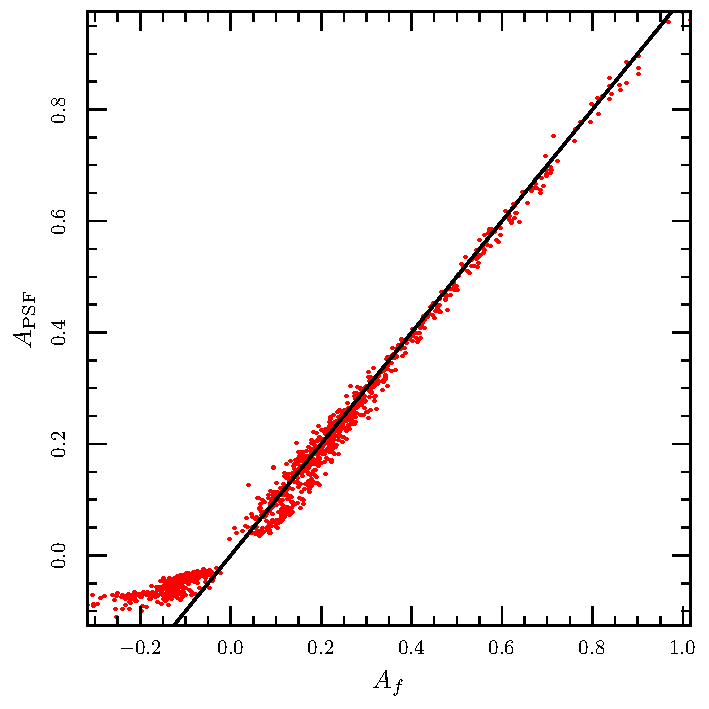
\includegraphics[width=\columnwidth]{acorr}
  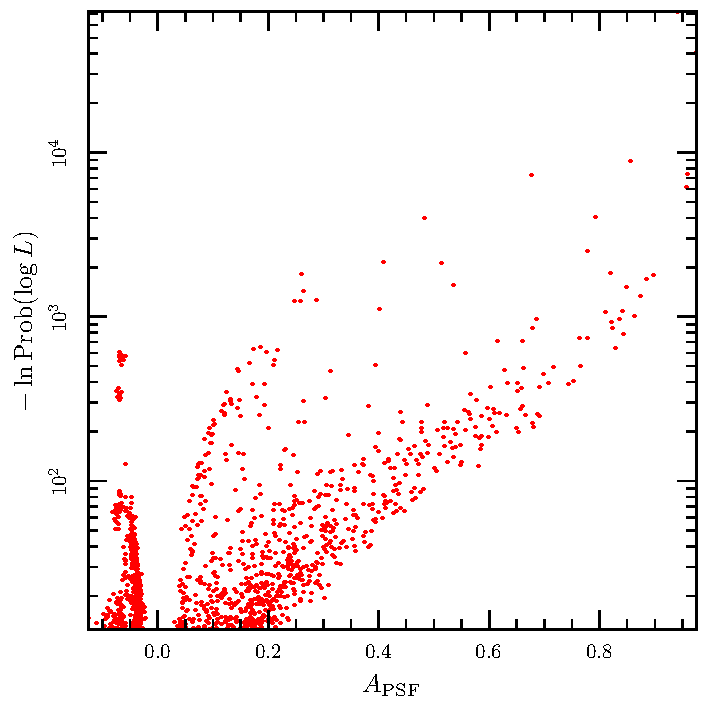
\includegraphics[width=\columnwidth]{asigcorr}
  \caption{Left: the correlation of the value $A_f$, determined from
    the means of the photon distributions, to the value of
    $A_\mathrm{PSF}$, determined from the maximum likelihood
    techinque.  Right: The values of $A_\mathrm{PSF}$ against the
    significance.}
  \label{fig:acorr}
\end{figure*}

Lorem Ipsum is simply dummy text of the printing and typesetting
industry. Lorem Ipsum has been the industry's standard dummy text ever
since the 1500s, when an unknown printer took a galley of type and
scrambled it to make a type specimen book. It has survived not only
five centuries, but also the leap into electronic typesetting,
remaining essentially unchanged. It was popularised in the 1960s with
the release of Letraset sheets containing Lorem Ipsum passages, and
more recently with desktop publishing software like Aldus PageMaker
including versions of Lorem Ipsum.

\begin{figure*}
  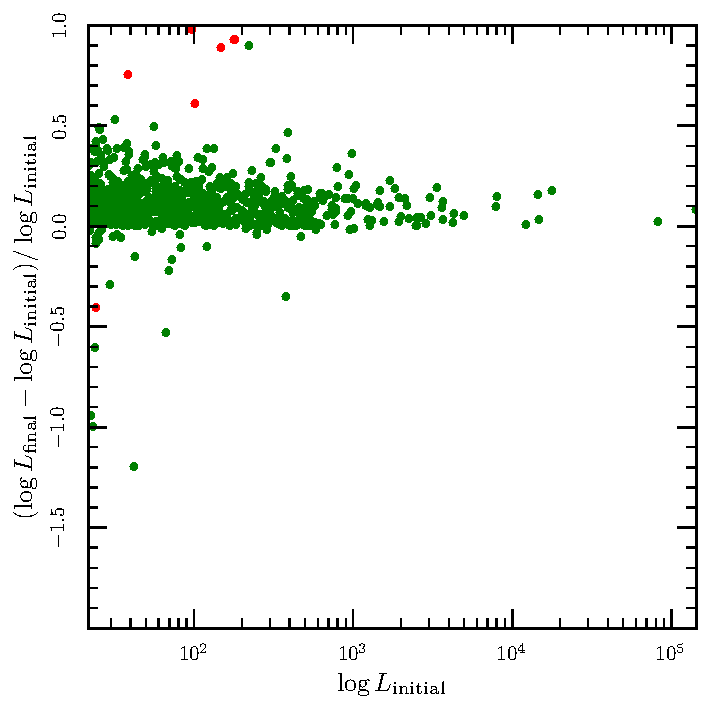
\includegraphics[width=\columnwidth]{changelogL}
  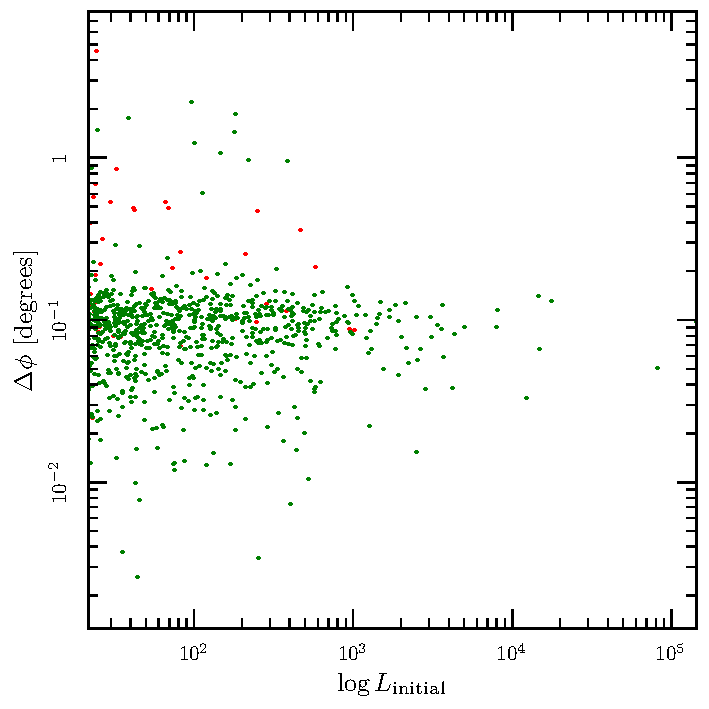
\includegraphics[width=\columnwidth]{change_position}
  \caption{Left: the relative change in $\log L$ during the position
    refinement.  Green is for sources whose positions moved less than
    one degree.  Red is for greater movement.  Right: the relative
    change in position during the position refinement.  Green is for
    sources whose positions likelihood increased.  Red is for those
    whose likelihood decreased.}
  \label{fig:position}
\end{figure*}


It is a long established fact that a reader will be distracted by the
readable content of a page when looking at its layout. The point of
using Lorem Ipsum is that it has a more-or-less normal distribution of
letters, as opposed to using 'Content here, content here', making it
look like readable English. Many desktop publishing packages and web
page editors now use Lorem Ipsum as their default model text, and a
search for 'lorem ipsum' will uncover many web sites still in their
infancy. Various versions have evolved over the years, sometimes by
accident, sometimes on purpose (injected humour and the like).

 Contrary to popular belief, Lorem Ipsum is not simply random text. It
has roots in a piece of classical Latin literature from 45 BC, making
it over 2000 years old. Richard McClintock, a Latin professor at
Hampden-Sydney College in Virginia, looked up one of the more obscure
Latin words, consectetur, from a Lorem Ipsum passage, and going
through the cites of the word in classical literature, discovered the
undoubtable source. Lorem Ipsum comes from sections 1.10.32 and
1.10.33 of "de Finibus Bonorum et Malorum" (The Extremes of Good and
Evil) by Cicero, written in 45 BC. This book is a treatise on the
theory of ethics, very popular during the Renaissance. The first line
of Lorem Ipsum, "Lorem ipsum dolor sit amet..", comes from a line in
section 1.10.32.

The standard chunk of Lorem Ipsum used since the 1500s is reproduced
below for those interested. Sections 1.10.32 and 1.10.33 from "de
Finibus Bonorum et Malorum" by Cicero are also reproduced in their
exact original form, accompanied by English versions from the 1914
translation by H. Rackham.

There are many variations of passages of Lorem Ipsum available, but
the majority have suffered alteration in some form, by injected
humour, or randomised words which don't look even slightly
believable. If you are going to use a passage of Lorem Ipsum, you need
to be sure there isn't anything embarrassing hidden in the middle of
text. All the Lorem Ipsum generators on the Internet tend to repeat
predefined chunks as necessary, making this the first true generator
on the Internet. It uses a dictionary of over 200 Latin words,
combined with a handful of model sentence structures, to generate
Lorem Ipsum which looks reasonable. The generated Lorem Ipsum is
therefore always free from repetition, injected humour, or
non-characteristic words etc.



\section{Results}

\begin{table*}
  \caption{The results for the ten most significant peaks in the 1~GeV map}
\label{tab:topten}
  \begin{tabular}{l|rrrrrrrrrrr}
    \hline
    Source & \multicolumn{1}{c}{RA} & \multicolumn{1}{c}{Dec}  & \multicolumn{1}{c}{$N_\mathrm{photons}$}  & \multicolumn{1}{c}{$\bar r^2$} & \multicolumn{1}{c}{$\bar f$} & \multicolumn{1}{c}{$S(r^2)$} & \multicolumn{1}{c}{$S(f)$} & \multicolumn{1}{c}{$A_f$} & \multicolumn{1}{c}{$TS_\mathrm{PSF}$} & \multicolumn{1}{c}{$A_\mathrm{PSF}$} &
    \multicolumn{1}{c}{$\ln P(TS)$} \\
    \hline

Vela             & $128.84$ & $-45.18$ & 172081 & $0.167$ & $0.507$ & $-478.9$ & $   9.7$ & $0.98$ & $156105.48$ & $0.96$ & $-78058.94$ \\ 
Geminga          & $ 98.48$ & $ 17.77$ &  90450 & $0.162$ & $0.503$ & $-352.3$ & $   3.4$ & $0.99$ & $ 84019.36$ & $0.98$ & $-42015.58$ \\ 
Crab             & $ 83.64$ & $ 22.02$ &  26547 & $0.189$ & $0.528$ & $-175.4$ & $  15.9$ & $0.92$ & $ 21557.26$ & $0.90$ & $-10783.85$ \\ 
PSR J1709-4429   & $257.42$ & $-44.48$ &  33105 & $0.258$ & $0.589$ & $-152.8$ & $  56.0$ & $0.73$ & $ 17373.25$ & $0.70$ & $ -8691.73$ \\ 
PSR J1836+5925   & $279.06$ & $ 59.43$ &  16605 & $0.163$ & $0.491$ & $-150.3$ & $  -4.0$ & $1.03$ & $ 15372.34$ & $0.97$ & $ -7691.22$ \\ 
3C 454.3	 & $343.50$ & $ 16.15$ &  14021 & $0.169$ & $0.511$ & $-135.7$ & $   4.6$ & $0.97$ & $ 12422.41$ & $0.96$ & $ -6216.15$ \\ 
PSR J0007.0+7303 & $  1.76$ & $ 73.05$ &  13610 & $0.212$ & $0.540$ & $-116.2$ & $  16.3$ & $0.88$ & $  9440.20$ & $0.83$ & $ -4724.90$ \\ 
PSR J2021.5+4026 & $305.39$ & $ 40.45$ &  30942 & $0.324$ & $0.665$ & $-107.0$ & $ 100.4$ & $0.52$ & $  8803.10$ & $0.51$ & $ -4406.32$ \\ 
PSR J1057-5226   & $164.49$ & $-52.46$ &   8222 & $0.227$ & $0.560$ & $ -85.8$ & $  18.9$ & $0.82$ & $  5301.47$ & $0.79$ & $ -2655.25$ \\ 
PSR J2021+3651	 & $305.26$ & $ 36.85$ &  22744 & $0.352$ & $0.699$ & $ -77.5$ & $ 103.8$ & $0.43$ & $  4612.93$ & $0.42$ & $ -2310.91$ \\ 
\end{tabular}
\end{table*}

\begin{figure*}
  \includegraphics[width=\textwidth]{fermi.png}
  \caption{Likelihood map with regions where $TS>25$, i.e. a
    significant detection of a source.  Because the point spead
    function is broader at 100~MeV than that at 1~GeV, the TS map at 100~MeV
    is fuzzier.}
\end{figure*}

\begin{figure*}
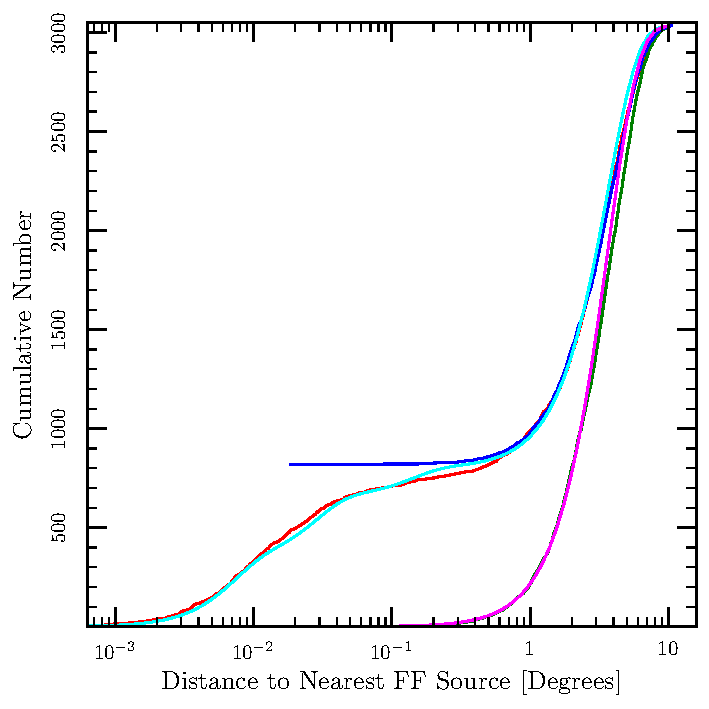
\includegraphics[width=\columnwidth]{cumfermi.pdf}
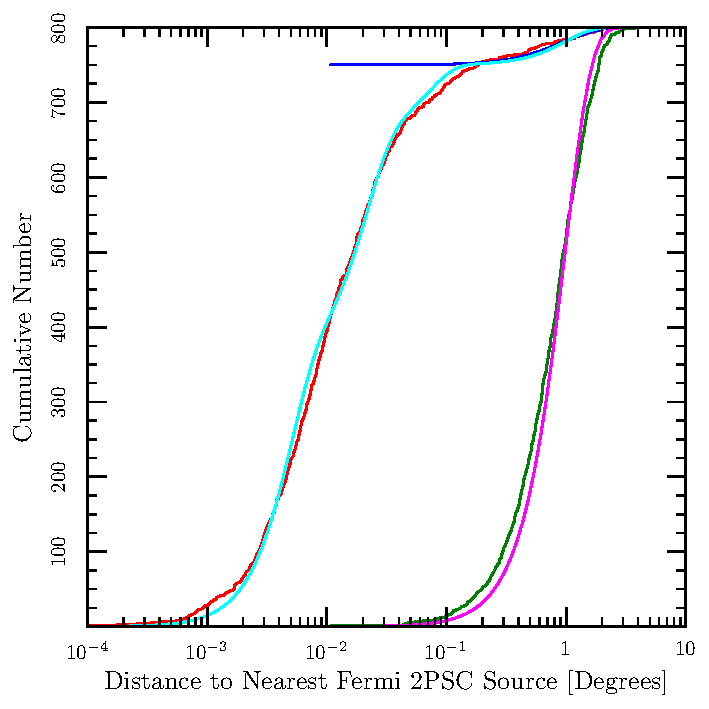
\includegraphics[width=\columnwidth]{cumff.pdf}

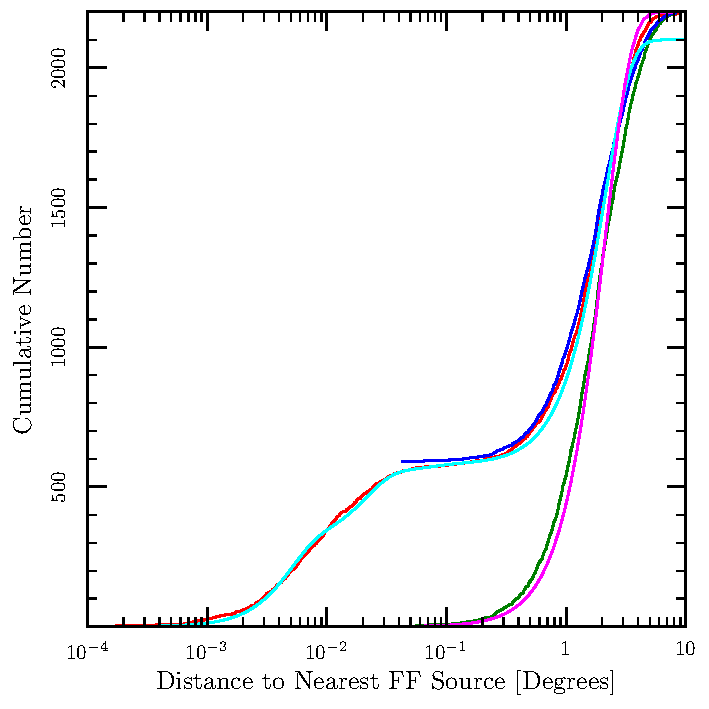
\includegraphics[width=\columnwidth]{cumfermi_hib.pdf}
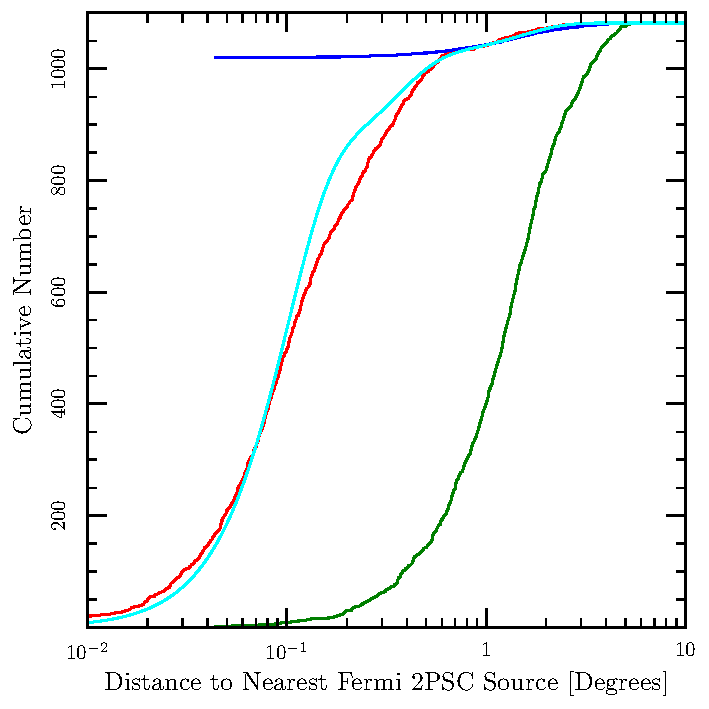
\includegraphics[width=\columnwidth]{cumff_hib.pdf}
\caption{The upper panels give the results for all sources and the lower panels have
  $|b|>10^\circ$.   Left: The distance from a Fermi 2PSC source to the nearest
  Fermi FAST source.  This demonstrates that Fermi FAST finds about
  half of the Fermi 2PSC sources.  Right: The distance from a Fermi
  FAST source to the nearest Fermi 2PSC source.  This demonstrates
  that ninety percent of the Fermi FAST sources are associated with
  sources in the FERMI 2PSC.  The red curve give the observed
  cumulative distribution of nearest distances.  The green curves give
  the cumulative distribution that one would expect if there were no
  associated between the Fermi FAST and Fermi 2PSC sources.  This is
  calculated by performing the same analysis as the red curves but
  with the Galactic coordinates inverted.  The blue curve yields the
  detection rate in the case of the left panels and the false positive
  rate for the right panels. The cyan and magneta curves are Rayleigh
  distributions that are fit to the observed distributions.  The
  typical positional error between associated 2PSC and FAST sources is
  four arcminutes.  }
\end{figure*}

\section*{Acknowledgments}

The software used in this paper is available at
\url{http://ubc-astrophysics.github.io}.  We used the VizieR Service,
the NASA ADS service, the Fermi Science Support Center, the astrometry.net
$k-d$~tree library, the HEALPix and HEALPy libraries and arXiv.org. This work
was supported by the Natural Sciences and Engineering Research Council
of Canada, the Canadian Foundation for Innovation, the British
Columbia Knowledge Development Fund and the Bertha and Louis Weinstein
Research Fund at the University of British Columbia.

\bibliography{fermi}
\bibliographystyle{mn2e}


\label{lastpage}

\end{document}

